\subsection{Lezione 14 17/10/2023}

\subsubsection{Bilanciamento All'inserimento in Albero R-B}

\begin{lstlisting}[language=Java]
	BilanciaInsSx(T)
		if !NIL(T->sx) and (!NIL(T->sx->sx) or !NIL(T->sx->dx)) then
			v = ViolazioneSxInsRB(T->sx,T->dx)
			Case V of :
				1: T = Caso1(T)
				2: T = Caso2(T)
				3: T= Caso3(T)
		return T
\end{lstlisting}

La violazione verifica se esiste una violazione di regola numero 4 (degli R-B), mandando il sottoalbero sinistro e destro rispettivamente all'interno di una funzione controllo che restituira il tipo di caso di violazione che stiamo riscontrando in quel sottoalbero.

\subsubsection{Controllo Violazione a Sinstra Inserimento R-B}

\begin{lstlisting}[language=Java]
	ViolazioneSxInsRB(s,d)
		v=0
		if s->col = R then
			if d->col = R then
				if s->sx->col = R or s->dx->col = R then
					v=1
			else if s->dx->col = R then
				v=2
			else if s->sx->col = R then
				v=3
		return v
\end{lstlisting}


\subsubsection{Risoluzione Violazione Inserimento a sinistra}
Quando andiamo ad inserire un nodo in un albero RB è facile violare le propietà, quindi andiamo a indentificare i 3 casi in cui avvengono e come andare a risolverli. Generalmente il problema principale è non rompere la proprieta 4. Per far si che non si rompa la proprieta diamo al nodo appena creato il colore rosso, che potrebbe compromettere i sottoalberi destro e sinistro.
\subsubsection{Caso 1}
Possiamo indentificare il \textbf{Caso 1}, osservando solamente se il figlio destro è un nodo rosso. La violazione puo avvenire sia sul sottoalbero sinistro del nodo sinistro della radice, sia nel destro.

\begin{figure}[H]
    \centering
    \begin{subfigure}[b]{0.35\textwidth}
        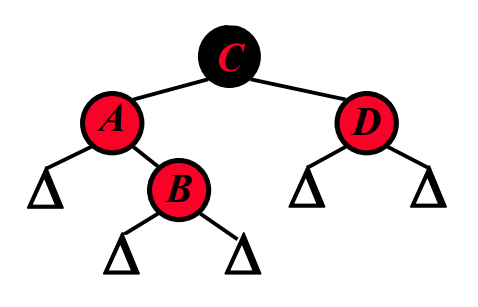
\includegraphics[width=\textwidth]{AlberoRBViolazioneCaso1-1} 
        \caption{Albero RB Caso 1 (n1)}
    \end{subfigure}
    \hfill
    \begin{subfigure}[b]{0.35\textwidth}
        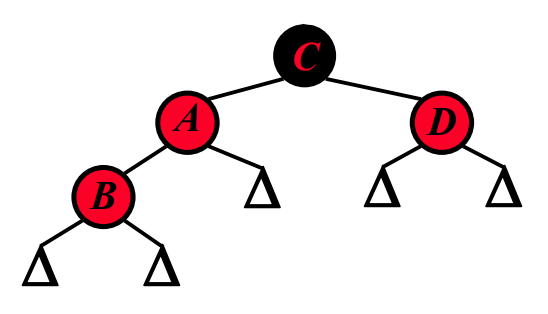
\includegraphics[width=\textwidth]{AlberoRBViolazioneCaso1-2} 
        \caption{Albero RB Caso 1 (n2)}
    \end{subfigure}
\end{figure}

Per corregere questa violazione andiamo a colorare la "radice" di rossa(anche se per convenziene dovrebbe essere nera), e poi di conseguenza andando a colorare i figli sinistri e destri di nero.
\begin{lstlisting}[language=Java]
	Caso1(T)
		T->dx->col=black;
		T->sx->col=black;
		T->col=red;
		return T;
\end{lstlisting}

In questo tipo di soluzione eliminiamo la violazione sui sottofigli, facciamo in modo che l'altezza nera sia rispettata in tutti i nodi, ma andiamo a "spostare" il problema verso l'alto, che poi verra corretto a cascata, fino eventualmente al nodo radice.

\begin{figure}[H]
    \centering
    \begin{subfigure}[b]{0.35\textwidth}
        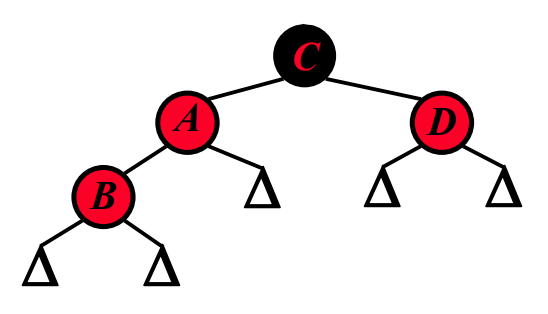
\includegraphics[width=\textwidth]{AlberoRBViolazioneCaso1-2} 
        \caption{Violazione Caso 1}
    \end{subfigure}
    \hfill
    \begin{subfigure}[b]{0.35\textwidth}
        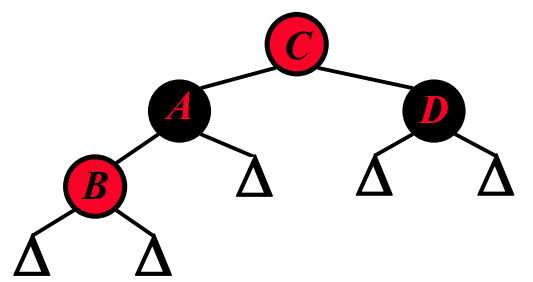
\includegraphics[width=\textwidth]{AlberoRBViolazioneCaso1-3} 
        \caption{Correzione Violazione}
    \end{subfigure}
\end{figure}


\subsubsection{Caso 2}

Il caso 2 (vedi foto) comporta il fatto che il \textbf{figlio destro} del sottoalbero su cui stiamo operando e \textbf{nero}. La strategia di risoluzione per il caso 2 prevede di far "ruotare" il problema a sinistra (quindi far salire di altezza la violazione) e far si che diventi caso 3, in questo modo andiam semplicemente a richiamare la strategia di risoluzione del caso 3.

\begin{figure}[H]
    \centering
    \begin{subfigure}[b]{0.35\textwidth}
        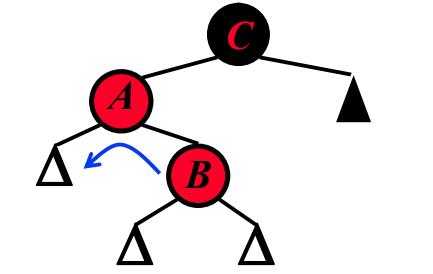
\includegraphics[width=\textwidth]{AlberoRBViolazioneCaso2-1} 
        \caption{Violazione Caso 1}
    \end{subfigure}
    \hfill
    \begin{subfigure}[b]{0.35\textwidth}
        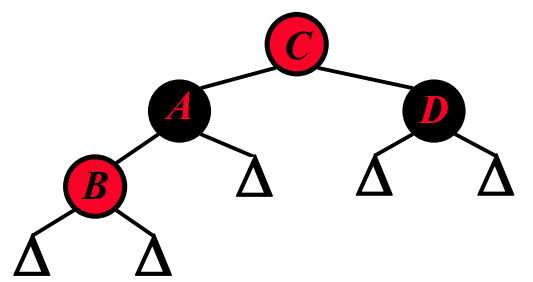
\includegraphics[width=\textwidth]{AlberoRBViolazioneCaso1-3} 
        \caption{Correzione Violazione}
    \end{subfigure}
\end{figure}

\begin{lstlisting}[language=Java]
	Caso2(T)
		T->sx = rotate(T->sx)
		t = Caso3(T)
		return T
\end{lstlisting}

\subsubsection{Caso 3}

Il caso 3, come nel caso 2, si verifica nel momento in cui, il figlio destro del sottoalbero su cui stiamo operando e nero. La differenza col caso 2 e che il figli del sottoalbero sinistro non sono entrambi rossi, ma il rosso si trova soltanto nel sottoalbero destro (come si nota in foto).
La strategia di risoluzione e dunque andare a ruotare sulla sinistra l'albero e scambiare i colori della radice e del figlo destro.

\begin{lstlisting}[language=Java]
	Caso3(T)
		T = rotazioneSx(T)
		T->col = N 
		T->dx->col = R
		return T
\end{lstlisting}

Ovviamente queste stesse violazioni sono possibili sul sottoalbero destro. Analogamente le soluzioni sono le stesse con opportune inversioni di nodi su cui devono essere fatte le operazioni.

\subsubsection{Delete Albero R-B}
Per la distruzione del nodo di un albero R-B ci vogliono molte piu accortezze della creazione poiche:
\begin{itemize}
	\item La distruzione di un nodo nero comporterebbe una failure nella proprieta 4 dell'altezza nera.
	\item Un nodo da disruggere potrebbe avere figli , quindi bisogna ragionare su come disporli e colorarli.
\end{itemize}

\textbf{Gli unici nodi da distruggere sono i nodi interni}.

L'elemento da sostituire cambiera colore in base a quale colore sia stato cancellato.

\begin{itemize}
	\item La distruzione di un nodo \textbf{rosso} comportera che il nodo acquistera il colore di nero.
	\item La distruzione di un nodo \textbf{nero} comportera che il nodo acquistera il colore di \textbf{doppio nero}, per non perdere la proprieta 4.
\end{itemize}

\begin{lstlisting}[language=Java]
	DeleteRB(T,k)
	if !NIL(T) then
		if T->key > k then
			T->sx = DeleteRB(T->sx,k)
			T = BilanciaDelsxRB(T)
		else if T->key < k then
			T->dx = DeleteRB(T->dx,k)
			T = BilanciaDeldxRB(T)
		else 
			T = DeleteRootRB(T)
	return T
\end{lstlisting}

Parallelamente alla delete degli AVL la funzione di DeleteRB hanno la stessa struttura di funzioni.

\begin{lstlisting}[language=Java]
	DeleteRootRB(T)
		if !NIL(T) then
			TMP = T
			if NIL(T->sx) then
				T = T->dx
				if TMP->col = N then	
					PropagateBlack(T)
			else if NIL(T->dx) then
				T = T->sx
				if TMP->col = N then
					PropagateBlack(T)
			else
				TMP = StaccaMinRB(T->dx, T)
				T = BilanciaDeldxRB(T)
			dealloca(TMP)
		return T
\end{lstlisting}